\clearpage
\section{Technische Grundlagen Zigbee}\label{sec:TechnischeGrundlagenZigbee}

\subsection{Netzaufbau und Topologie}\label{subsec:NetzaufbauundTopologie}
\todo[inline]{Welchen Aufbau? Welche Art von Mesh? Welche Nodetypen gibt es? Welche typischen Eigenschaften besitzt das Protokoll?}


\subsubsection{Topologie}\label{subsubsec:Topologie}


\begin{figure}[h]
	\centering
	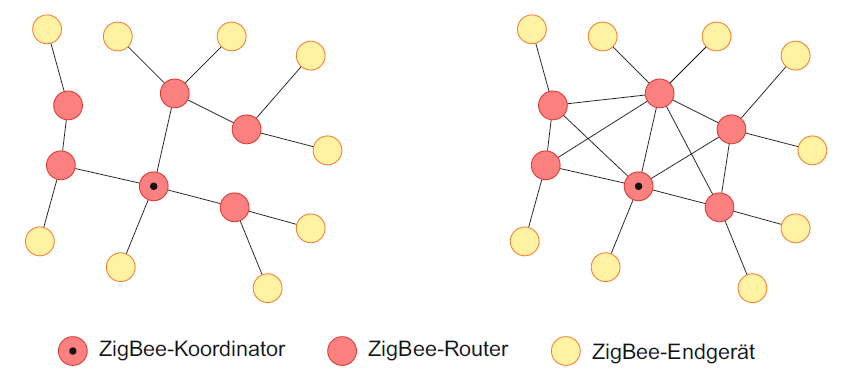
\includegraphics[width=0.8\textwidth]{Zigbee_Netztopologie.png}
	\caption{Netzwerktopologien Zigbee \cite{markus_krause_rainer_konrad_drahtlose_2014}}
	\label{fig:NetzwerktopologienZigbee}
\end{figure}

\subsubsection{Nodetypen}\label{subsubsec:Nodetypen}
\paragraph{Zigbee Coordinator}\label{para:ZigbeeCoordinator}

\paragraph{Zigbee Router}\label{para:ZigbeeRouter}

\paragraph{Zigbee End Device}\label{para:ZigbeeEndDevice}





\subsection{Zigbee Protokoll Stack}\label{subsec:ZigbeeProtokollStack}
\todo[inline]{Erläuterung des Protokoll Stacks. Möglichst viel Grafiken und nur so viel als nötig Prosa.}



\begin{figure}[h]
	\centering
	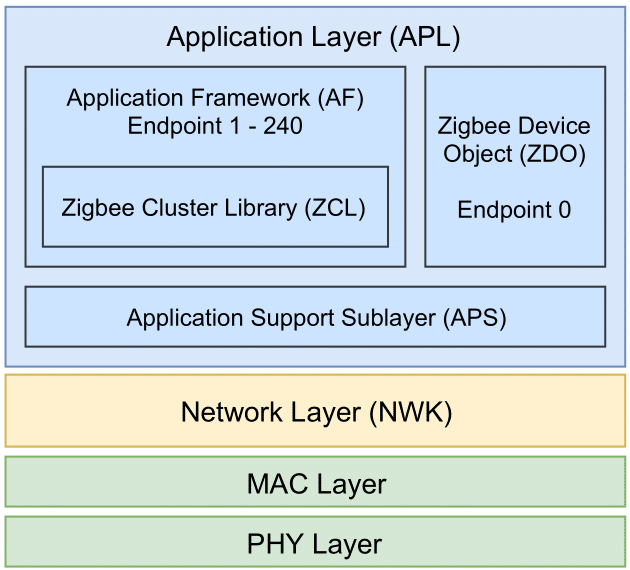
\includegraphics[width=\textwidth]{Zigbee_Architektur.png}
	\caption{Architektur des Zigbee Protokoll Stacks \cite{markus_krause_rainer_konrad_drahtlose_2014}}
	\label{fig:ArchitekturdesZigbeeProtokollStacks}
\end{figure}

\subsubsection{MAC und PHY Layer}\label{subsubsec:MACundPHYLayer}

\subsubsection{Network Layer}\label{subsubsec:Network Layer}

\paragraph{Routing}\label{par:Zigbee Routing}
\todo[inline]{Route discovery packets.}
\todo[inline]{Routing table}






\subsubsection{Application Support Sublayer (APS)}\label{subsubsec:ApplicationSupportSublayer}


\subsubsection{Application Layer}\label{subsubsec:ZigbeeApplicationLayer}

\paragraph{Zigbee Cluster Library (ZCL)}\label{par:ZigbeeClusterLibrary}

\paragraph{Endpunkte}\label{par:ZigbeeEndpunkte}





\subsection{Zigbee Software Development Kit}\label{subsec:ZigbeeSoftwareDevelopmentKit}
\todo[inline]{Eingesetzte SDK und deren Aufbau beschreiben. Allenfalls die wichtigsten API Funktionen genauer erläutern.}
